\documentclass[11pt,a4paper]{article}

% =========================
% Packages
% =========================
\usepackage[T1]{fontenc}
\usepackage[utf8]{inputenc}
\usepackage[english]{babel}

\usepackage{geometry}
\geometry{margin=1in}

\usepackage{lmodern}
\usepackage{microtype}

\usepackage{amsmath,amssymb,amsthm,mathtools,bm}
\usepackage{bbm}          % \mathbbm{1}
\usepackage{booktabs}
\usepackage{siunitx}
\sisetup{detect-all,group-separator={,},group-minimum-digits=4}

\usepackage{graphicx}
\usepackage{adjustbox}
\usepackage{subcaption}

\usepackage{xcolor}
\usepackage{hyperref}
\usepackage{cleveref}
\usepackage{url}          % \nolinkurl handles underscores safely

% Enforce figure ordering
\usepackage{placeins}     % provides \FloatBarrier

% Optional (compact lists)
\usepackage{enumitem}
\setlist{noitemsep,topsep=2pt}

% TikZ for pipeline diagram
\usepackage{tikz}
\usetikzlibrary{arrows.meta,positioning,fit,backgrounds,calc}

% =========================
% Macros
% =========================
\providecommand{\mb}[1]{#1}
\renewcommand{\mb}[1]{\bm{#1}}
\providecommand{\mc}[1]{#1}
\renewcommand{\mc}[1]{\mathcal{#1}}
\providecommand{\1}{}
\renewcommand{\1}{\mathbbm{1}}
\newcommand{\BetP}{\mathrm{BetP}}
\providecommand{\E}{\mathbb{E}}
\renewcommand{\E}{\mathbb{E}}

\newtheorem{prop}{Proposition}

% Graphics path (paper assets)
% NOTE: Experimental artifacts are generated under Common_code/results/outlier_plots/.
\graphicspath{{./}{results/}{results/outlier_plots/}{Common_code/results/}{Common_code/results/outlier_plots/}}

% Safe figure include (no hard-stop compile if a file is missing)
\newcommand{\safeincludegraphics}[2][]{%
  \IfFileExists{#2}{\includegraphics[#1]{#2}}{%
    \fbox{\parbox{0.95\linewidth}{%
      \textbf{Missing file:} \nolinkurl{#2}\\
      Upload the file to the Prism project or fix the filename/path.%
    }}%
  }%
}

% =========================
% Title
% =========================
\title{DSGD-Auto: Automatically Induced Rules for Dempster--Shafer Fusion\\
Readable Combined-Condition Explanations}

\author{Sargis Vardanyan \and Hayk Tarkhanyan \and Ashot Harutyunyan}
\date{September 2025}

\begin{document}
\maketitle

% ============================================================
\begin{abstract}
Dempster--Shafer Gradient Descent (DSGD) learns Dempster--Shafer mass vectors and outputs class probabilities via the pignistic transformation while keeping an explicit ``I don't know'' mass $m(\Theta)$.
We present \textbf{DSGD-Auto}, a simple two-stage pipeline for tabular data: (i) automatically induce an interpretable rule base and freeze its logic, then (ii) learn only one singleton+$\Theta$ mass vector per rule on the simplex.
At inference time, the model activates the fired rules, fuses their learned masses, and outputs both calibrated probabilities and the remaining ignorance mass $m_\Theta(x)$.

We study three inducers that produce rule bases with very different densities: STATIC (many short rules), RIPPER/IREP (compact rule lists), and FOIL-style greedy growth (intermediate).
Our main empirical finding is that uncertainty behavior is strongly controlled by fusion depth: when many overlapping rules fire, repeated Dempster fusion can collapse $m_\Theta(x)$ and make the model appear overconfident even if individual rules are cautious.
Alongside standard calibration metrics (ECE/NLL), we therefore report DS-specific diagnostics (fusion depth and per-rule vs.\ fused ignorance), and we provide an inspection-only \emph{combined condition} that summarizes influential fired literals into a single human-readable explanation.
\end{abstract}

% ============================================================
\begin{figure}[t]
\centering
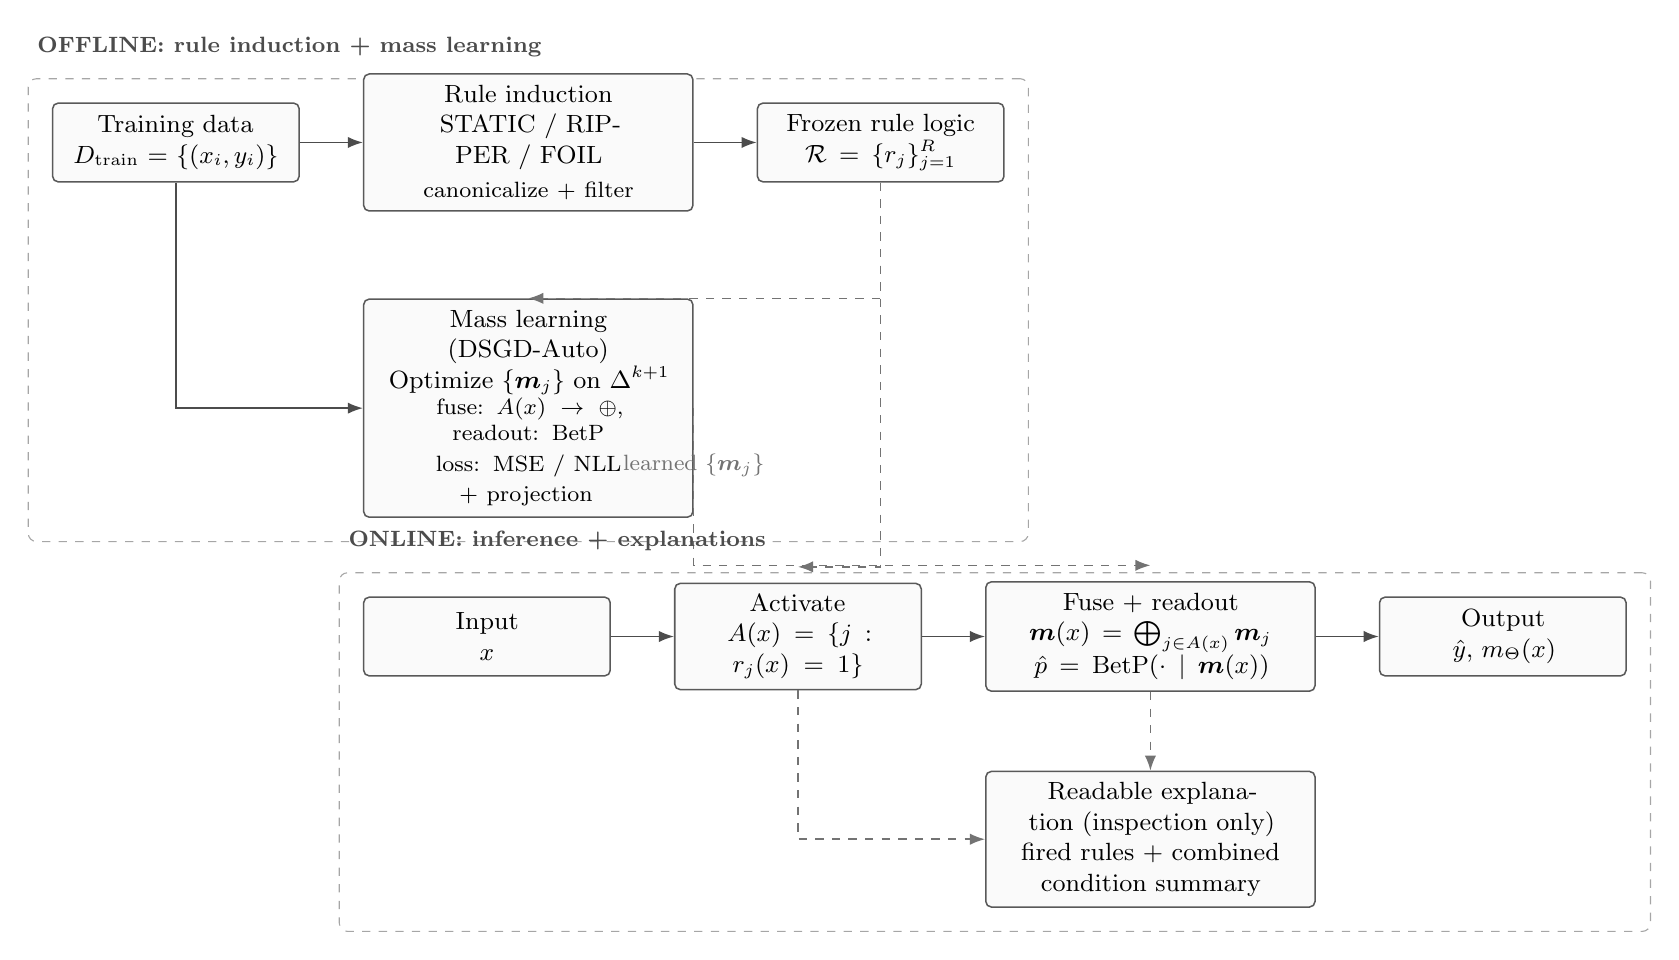
\begin{tikzpicture}[
  font=\small,
  node distance = 6mm and 8mm,
  block/.style={draw=black!65, line width=0.55pt, rounded corners=2pt,
                align=center, inner sep=4pt, minimum height=10mm, fill=black!2},
  blockwide/.style={block, text width=3.90cm},
  blocknarrow/.style={block, text width=2.85cm},
  arrow/.style={-Latex, line width=0.55pt, draw=black!70},
  darrow/.style={-Latex, line width=0.55pt, draw=black!55, dashed},
  phase/.style={draw=black!35, dashed, rounded corners=3pt, inner sep=3mm}
]

% ===== OFFLINE (training) =====
\node[blocknarrow] (train) {Training data\\$D_{\mathrm{train}}=\{(x_i,y_i)\}$};
\node[blockwide, right=of train] (induce) {Rule induction\\STATIC / RIPPER / FOIL\\\vspace{0.5mm}\footnotesize canonicalize + filter};
\node[blocknarrow, right=of induce] (rules) {Frozen rule logic\\$\mc{R}=\{r_j\}_{j=1}^{R}$};

\node[blockwide, below=11mm of induce] (learn) {Mass learning (DSGD-Auto)\\Optimize $\{\mb{m}_j\}$ on $\Delta^{k+1}$\\\footnotesize fuse: $A(x)\rightarrow \oplus$,\ \ readout: $\BetP$\\\footnotesize loss: MSE / NLL + projection};

% arrows (offline)
\draw[arrow] (train) -- (induce);
\draw[arrow] (induce) -- (rules);
\draw[arrow] (train) |- (learn.west);
\draw[darrow] (rules) |- (learn.north);

% ===== ONLINE (inference) =====
\node[blocknarrow, below=29mm of learn.west, anchor=west] (xin) {Input\\$x$};
\node[blocknarrow, right=of xin] (act) {Activate\\$A(x)=\{j:r_j(x)=1\}$};
\node[blockwide, right=of act] (fuse) {Fuse + readout\\$\mb{m}(x)=\bigoplus_{j\in A(x)} \mb{m}_j$\\$\hat p=\BetP(\cdot\mid \mb{m}(x))$};
\node[blocknarrow, right=of fuse] (out) {Output\\$\hat y,\, m_\Theta(x)$};

\node[blockwide, below=10mm of fuse] (explain) {Readable explanation (inspection only)\\fired rules + combined condition summary};

\draw[arrow] (xin) -- (act);
\draw[arrow] (act) -- (fuse);
\draw[arrow] (fuse) -- (out);
\draw[darrow] (act) |- (explain.west);
\draw[darrow] (fuse) -- (explain);

% shared artifacts (cross-phase)
\draw[darrow] (rules.south) |- ([yshift=2mm]act.north);
\draw[darrow] (learn.east) |- node[pos=0.25, above, font=\footnotesize, text=black!55]{learned $\{\mb{m}_j\}$} ([yshift=2mm]fuse.north);

% phase boxes (background)
\begin{pgfonlayer}{background}
\node[phase, fit=(train)(rules)(learn)] (offline) {};
\node[phase, fit=(xin)(out)(explain)] (online) {};
\end{pgfonlayer}

% phase labels
\node[anchor=south west, font=\footnotesize\bfseries, text=black!70]
  at ([yshift=1.5mm]offline.north west) {OFFLINE: rule induction + mass learning};
\node[anchor=south west, font=\footnotesize\bfseries, text=black!70]
  at ([yshift=1.5mm]online.north west) {ONLINE: inference + explanations};

\end{tikzpicture}
\caption{DSGD-Auto pipeline. Rule logic is induced once and frozen; only singleton+$\Theta$ masses are learned on the simplex. At inference, fired rules are fused and read out via the pignistic transformation to obtain calibrated probabilities and the ignorance mass $m_\Theta(x)$. For interpretability, we also provide an inspection-only combined-condition summary.}
\label{fig:dsgd-auto-pipeline}
\end{figure}

% ============================================================
\section{Introduction}
% ============================================================
Rule-based models remain attractive for tabular decision making when auditability matters: a human can inspect the logic, verify constraints, and trace which conditions triggered a decision. However, most rule learners output hard votes or heuristic scores, and probability estimates (when present) are often weakly justified and poorly calibrated. In high-stakes settings, accuracy alone is insufficient: a usable system should expose both reliable probabilities and a principled ``I don't know'' signal.

Dempster--Shafer (DS) theory represents uncertainty by a mass function with an explicit uncommitted mass $m(\Theta)$ and supports evidence fusion; probabilities are obtained via the pignistic transformation \cite{Shafer1976,Smets2005}.

\paragraph{DSGD (Pe\~nafiel et al.).}
DSGD \cite{Penafiel2020} treats each evidence source (e.g., a rule) as a learnable mass assignment function that outputs singleton+$\Theta$ masses.
For an input $x$, we evaluate which rules fire, fuse the masses of the active set $A(x)$ sequentially using Dempster's normalized rule, and convert the fused mass $\mb{m}(x)$ into class probabilities via the pignistic transformation.
Training optimizes the per-source masses (under simplex constraints), while the set of sources itself is assumed to be given.

\paragraph{DSGD++ (Hayk Tarkhanyan, Ashot Harutyunyan).}
DSGD++ \cite{Tarkhanyan2025} improves DSGD's practical stability by changing how masses are initialized and constrained during learning.
In our implementation this corresponds to a confidence-guided initialization (representativeness $\times$ purity) followed by stable optimization of per-rule mass vectors, while keeping DS fusion itself unchanged.

\paragraph{What DSGD-Auto adds.}
In DSGD and DSGD++, the evidence sources (rules) are an input to the method.
DSGD-Auto makes evidence-source design explicit: we automatically induce a \emph{frozen} rule base and then learn only the per-rule singleton+$\Theta$ masses.
This separates \emph{rule logic} (human-readable and fixed after induction) from \emph{uncertainty calibration} (learned masses), and lets us study how rule induction changes DS fusion dynamics.

\paragraph{Rule induction variants (STATIC/RIPPER/FOIL).}
We compare three implementation-grounded generators:
\begin{itemize}
\item \textbf{STATIC (baseline, brute force).} A large pool of candidate literals is created from quantile thresholds for numeric features and frequent equality tests for categorical features, and expanded into low-order conjunctions (singletons/pairs/triples). In our codebase, these rules are \emph{unlabeled predicates}: their class support is expressed only through the learned mass vector. This yields many short rules: each rule is easy to read, but typically weak on its own, and a single instance may activate many rules (deep fusion).
\item \textbf{RIPPER/IREP (rule list).} A separate-and-conquer learner that greedily grows a rule, then prunes it (reduced-error pruning), producing a compact set of longer, class-labeled rules \cite{Cohen1995}. Fewer fired rules imply shallower DS fusion and typically more stable uncertainty behavior.
\item \textbf{FOIL-style growth.} Greedy growth of class-labeled conjunctions driven by FOIL gain \cite{Quinlan1990} without RIPPER-style pruning. This tends to produce an intermediate regime: fewer rules than STATIC, often longer rules than STATIC, and moderate fusion depth.
\end{itemize}

\paragraph{Fusion, readout, and diagnostics.}
At inference time, activation is computed by evaluating all \emph{unique} literals and then marking a rule as active when all its literals are satisfied (vectorized via a literal-to-rule incidence matrix).
Active rules are fused strictly by Dempster during training; at inference we additionally expose Yager's conflict transfer as an \emph{ablation/diagnostic} \cite{Yager1987}.
The final output is a probability vector (pignistic readout) plus explicit uncertainty $m_\Theta(x)$.

\paragraph{Interpretability: fired rules and a ``combined condition''.}
The primary explanation is the set of fired rules and their learned masses.
For readability, we also compute a post-hoc \emph{combined condition} (explanation-only): fired rules are weighted by how strongly they support the \emph{predicted} class (positive weight for agreeing rules, negative weight for conflicting rules; optionally scaled by a rule-level statistic such as precision for inspection only); only positive weight is distributed across the rule's literals; per-feature constraints are then merged (for a fixed feature, we keep the strongest lower bound for ``$>$'' and the strongest upper bound for ``$<$'', and for ``$==$'' we keep the value with the highest total weight), yielding a single conjunction.
This combined condition is not used for inference and is not logically equivalent to the full fired rule set; it is a compact summary intended to answer ``what constraints supported this decision?''.

\paragraph{Why rule-base density matters.}
Dense bases (STATIC) increase fusion depth, which can amplify conflict sensitivity under Dempster normalization and collapse fused ignorance $m_\Theta(x)$ even when individual rules are cautious.
We therefore report calibration (ECE/NLL) together with DS-specific diagnostics (mean per-rule ignorance vs.\ mean fused ignorance, and fusion depth), since these expose failure modes that accuracy can hide.

% ============================================================
\section{Preliminaries: DS masses, fusion, and probability readout}
% ============================================================
Let $\Omega=\{1,\dots,k\}$ be the set of classes and $\Theta=\Omega$ the frame of discernment.

\subsection{Singleton+\texorpdfstring{$\Theta$}{Theta} masses}
Each rule $r_j$ has a learnable mass vector
\[
\mb{m}_j=\big(m_{j,1},\dots,m_{j,k},m_{j,\Theta}\big),
\quad
m_{j,c}\ge 0,\quad \sum_{c=1}^k m_{j,c}+m_{j,\Theta}=1.
\]
We restrict masses to singleton hypotheses plus ignorance. This matches the common efficient setting used in DSGD-like implementations and keeps fusion differentiable and cheap.

\subsection{Dempster fusion (normalized)}
Given two masses $m$ and $m'$, define conflict for singleton+$\Theta$ masses by
\[
\kappa = \sum_{\substack{a\neq b\\ a,b\in\Omega}} m_a m'_b.
\]
Dempster's normalized combination is
\[
(m\oplus m')_c
=
\frac{m_c m'_c + m_c m'_{\Theta} + m_{\Theta} m'_c}{1-\kappa},
\qquad
(m\oplus m')_{\Theta}
=
\frac{m_{\Theta}m'_{\Theta}}{1-\kappa}.
\]
In implementation, $1-\kappa$ is clipped away from zero for numerical stability when conflict is extreme.

\subsection{(Ablation) Yager conflict transfer}
A robustness alternative transfers conflict to ignorance without renormalization \cite{Yager1987}:
\[
m^{Y}_c = m_c m'_c + m_c m'_{\Theta} + m_{\Theta} m'_c,
\qquad
m^{Y}_{\Theta} = m_{\Theta}m'_{\Theta} + \kappa.
\]
We use Yager fusion only to evaluate conflict sensitivity; the core training setup remains Dempster-based.

\subsection{Pignistic probabilities}
We output class probabilities via the pignistic transformation \cite{Smets2005}. For singleton+$\Theta$ masses, the probability readout can be written as
\[
\hat p_c(x)=\BetP(c\mid \mb{m}(x)) = m_c(x) + m_{\Theta}(x)\,\pi_c,
\qquad
\pi_c \ge 0,\ \sum_{c=1}^k \pi_c = 1.
\]
The classical choice is the uniform prior $\pi_c=\tfrac{1}{k}$.
\textit{Implementation note (Common\_code).} In our experiments we use an \emph{inverse-frequency} prior to reduce the effect of severe imbalance:
\[
\pi_c = \frac{n_c^{-\alpha}}{\sum_{b=1}^k n_b^{-\alpha}},
\]
where $n_c$ is the class count in the training split and $\alpha\in[0,1]$ (uniform is recovered at $\alpha=0$).

% ============================================================
\section{Rule induction as evidence-source design}
% ============================================================
Let $D=\{(x_i,y_i)\}_{i=1}^n$ with $x_i\in\mathbb{R}^d$ and $y_i\in\Omega$.
A rule set $\mc{R}=\{r_j\}_{j=1}^R$ defines Boolean predicates $f_j(x)\in\{0,1\}$;
the active set is $A(x)=\{j: f_j(x)=1\}$.

\subsection{Rule representation (literals)}
A rule body is a conjunction of literals,
\[
r_j(x)=\1\!\Big[\bigwedge_{\ell\in\mc{L}(r_j)} \ell(x)\Big],
\]
with literals typically of the form $x_t\le \tau$, $x_t > \tau$, or (for categorical features) $x_t = v$.

\subsection{How literals are merged when rules are combined}
Because rules are conjunctions, combining (or growing) rules corresponds to intersecting their constraints.
In the implementation, we merge literals feature-wise to avoid contradictions and to keep a stable canonical form.

\paragraph{Numeric features.}
For each numeric feature $t$, we maintain an interval constraint of the form
\[
x_t \in (L_t, U_t],
\]
where $L_t$ may be $-\infty$ and $U_t$ may be $+\infty$.
A literal $x_t \le \tau$ updates the upper bound $U_t \leftarrow \min(U_t,\tau)$.
A literal $x_t > \tau$ updates the lower bound $L_t \leftarrow \max(L_t,\tau)$.
If after an update $L_t \ge U_t$, the conjunction is infeasible and the candidate rule is discarded.

\paragraph{Categorical features.}
For a categorical feature $t$, literals are equalities $x_t=v$.
Combining literals on the same feature keeps the value if consistent; if two different values appear, the conjunction is infeasible.

\paragraph{Note on explanation strings.}
The code may store a ``combined condition string'' for readability, but the model-side matching uses the merged canonical constraints above (not the raw concatenated string).

\subsection{Combined rule explanations (inspection-only)}
\label{sec:combined-rule-expl}
In addition to listing fired rules, our implementation can output a compact \emph{combined condition} for a single instance.
This combined condition is constructed purely for interpretability and does \textbf{not} affect prediction.

\paragraph{What is combined.}
The inspector first computes the DS prediction (Dempster or Yager at inference time) and then assigns each fired rule an explanation weight.
Only positively supporting rules contribute their literals. Literal contributions are aggregated into a single conjunction by grouping identical $(\texttt{feature},\texttt{operator})$ keys and selecting a representative value:
for numeric thresholds, ``$>$'' keeps the maximum threshold and ``$<$'' keeps the minimum threshold (tightening the interval);
for equality constraints ``$==$'' a weighted mode is selected (a summary choice).

\paragraph{What this means (and what it does \emph{not} mean).}
Because the combined condition is built from \emph{weighted} contributions (and because different equalities on the same feature cannot be jointly satisfied),
the combined condition should be interpreted as a \emph{prediction-conditioned summary} of influential literals, not as a logically equivalent representation of all fired rules.
This design is deliberate: it is meant to help a user quickly inspect which feature constraints supported the decision, without reading hundreds of rules.

\subsection{Duplicate filtering and diversity control}
Dense split grids (e.g., quantile thresholds) can create many near-duplicate univariate rules.
To prevent an explosion of redundant candidates, we apply a \emph{diversity filter} based on coverage overlap.
For each rule $r$, let $S(r)\subseteq\{1,\dots,n\}$ be the set of training indices it covers.
We discard a new candidate $r$ if there exists a kept rule $r'$ with high Jaccard similarity
\[
J(r,r')=\frac{|S(r)\cap S(r')|}{|S(r)\cup S(r')|}>\tau,
\]
using $\tau=0.85$ by default (configurable).
When two candidates are near-duplicates, we keep the one with higher estimated quality (rule confidence/purity or gain, depending on the inducer).

\subsection{Candidate thresholds and greedy growth (FOIL-style)}
For a numeric feature $t$, candidate thresholds are taken from a fixed quantile grid $Q$ on the training split
(default $Q=\{0.05,0.10,\dots,0.95\}$). Each threshold $\tau=Q_q(x_t)$ induces two literals: $x_t\le\tau$ and $x_t>\tau$.
FOIL-style rule growth greedily adds the literal that maximizes a gain criterion \cite{Quinlan1990} and stops when the best gain falls below \texttt{min\_gain}.


\subsection{Inducers: STATIC vs.\ RIPPER vs.\ FOIL}
We use three families of inducers, intentionally chosen to produce different rule-base densities:
\begin{itemize}
\item \textbf{STATIC:} generates many short, mostly one--three-literal statistical rules. It is fast but often produces dense rule bases.
\item \textbf{RIPPER/IREP:} a separate-and-conquer rule-list learner that grows and prunes rules and defines a default decision when no rule fires \cite{Cohen1995}. In practice it yields sparse rule lists.
\item \textbf{FOIL-style growth:} greedily adds literals that improve a gain-like criterion \cite{Quinlan1990}, typically producing moderate rule sets with longer conjunctions than STATIC.
\end{itemize}

\subsection{Why inducer choice matters in DS fusion}
DS fusion repeatedly combines masses over the active set $A(x)$. If an inducer yields dense rule bases, then typical $|A(x)|$ is larger and fusion depth increases. This can:
(i) amplify conflict sensitivity under Dempster normalization, and
(ii) collapse the fused ignorance mass $m_\Theta(x)$ even when individual rules have high $m_{j,\Theta}$.
Sparse rule lists (RIPPER/FOIL) often reduce fusion depth and can preserve meaningful ignorance.

\begin{figure}[t]
\centering
\safeincludegraphics[width=0.95\linewidth]{rule_counts_pastel.png}
\caption{Rule-base density diagnostics (pastel style): number of rules and average rule length by dataset and inducer.
Dense rule bases imply deeper evidence fusion and can trigger fusion-driven ignorance collapse under normalized DS fusion.}
\label{fig:rule-density}
\end{figure}

\begin{table}[t]
\centering
\caption{Rule-base density snapshot from \texttt{Common\_code} runs (train-induced rules).
Counts may vary slightly with the seed and duplicate-filter threshold.
Rule length is the average number of literals (conjuncts) per rule body.}
\label{tab:rule-density-snapshot}
\begin{tabular}{l S[table-format=4.0] S[table-format=3.1] S[table-format=3.0] S[table-format=3.1] S[table-format=3.0] S[table-format=3.1]}
\toprule
Dataset & \multicolumn{2}{c}{STATIC} & \multicolumn{2}{c}{RIPPER} & \multicolumn{2}{c}{FOIL} \\
\cmidrule(lr){2-3} \cmidrule(lr){4-5} \cmidrule(lr){6-7}
 & {$R$} & {$\mathbb{E}[|r|]$} & {$R$} & {$\mathbb{E}[|r|]$} & {$R$} & {$\mathbb{E}[|r|]$} \\
\midrule
adult & 392 & 2.27 & 304 & 4.66 & 614 & 5.45 \\
bank-full & 800 & 2.63 & 267 & 4.85 & 417 & 5.31 \\
BrainTumor & 853 & 2.52 & 23 & 2.83 & 60 & 4.32 \\
breast-cancer-wisconsin & 559 & 2.56 & 18 & 1.33 & 42 & 2.17 \\
df\_wine & 542 & 2.64 & 104 & 4.29 & 164 & 4.78 \\
german & 714 & 2.61 & 61 & 3.49 & 141 & 4.55 \\
SAheart & 796 & 2.63 & 25 & 3.12 & 78 & 4.91 \\
gas\_drift & 2000 & 1.20 & 114 & 4.22 & 169 & 4.30 \\
\bottomrule
\end{tabular}
\end{table}

\noindent\textbf{Key observations from Table~\ref{tab:rule-density-snapshot}:}
\begin{itemize}
\item \textbf{STATIC} produces the densest rule bases (392--2000 rules) with shortest average rule length (1.20--2.64 literals), leading to deep fusion chains and high risk of ignorance collapse.
\item \textbf{RIPPER} produces the sparsest rule bases (18--304 rules) with moderate length (1.33--4.85 literals), reducing fusion depth and preserving uncertainty.
\item \textbf{FOIL} lies between STATIC and RIPPER (42--614 rules) with longer rules on average (2.17--5.45 literals), offering a balance between coverage and fusion depth.
\item Extreme cases: \texttt{gas\_drift} STATIC has 2000 rules but very short rules (1.20 avg), while \texttt{breast-cancer-wisconsin} RIPPER has unusually short rules (1.33 avg) due to a simple feature space.
\end{itemize}

% ============================================================
\section{Method: DS mass learning on induced rules}
% ============================================================

\subsection{Instance-level fusion}
We initialize the ``empty evidence'' mass as pure ignorance,
\[
\mb{m}^{(0)}=(0,\dots,0,1),
\]
and fuse all active rules:
\[
\mb{m}(x)=\bigoplus_{j\in A(x)} \mb{m}_j,
\quad\text{or}\quad
\mb{m}^{Y}(x)=\bigoplus\nolimits^{Y}_{j\in A(x)} \mb{m}_j\ \text{(ablation)}.
\]
If $A(x)=\varnothing$, we keep $\mb{m}(x)=\mb{m}^{(0)}$.
In our implementation, training strictly uses Dempster's rule (non-Dempster combination rules are rejected in training mode); Yager is used only for inference-time diagnostics.

\subsection{What is learned vs.\ fixed}
Rule bodies $\mc{L}(r_j)$ are frozen after induction.
Only the per-rule masses $\{\mb{m}_j\}_{j=1}^R$ are trained, so interpretability stays in the rule logic while calibration is delegated to masses.

\subsection{Loss and optimization}
We compute pignistic probabilities $\hat p(x)$ and train masses by minimizing
\[
\mc{L} = \frac{1}{n}\sum_{i=1}^n \|\hat p(x_i)-e_{y_i}\|_2^2
\]
(MSE on probabilities) with optional class weighting. Cross-entropy/NLL is supported as an alternative but is mainly used as an evaluation diagnostic.
After each optimizer step, each $\mb{m}_j$ is projected back onto the $(k+1)$-simplex (nonnegativity and unit sum).

\subsection{DSGD++-style initialization (adapted)}
DSGD++ proposes a confidence-based initialization to reduce training time and uncertainty, using data representativeness and class centroids \cite{Tarkhanyan2025}.
In our codebase, this corresponds to initializing each evidence source with:
(i) a dominant singleton mass $\alpha_1$ on the most likely class,
(ii) small $\epsilon$ masses on other singletons, and
(iii) remaining mass on $\Theta$:
\[
m_{j,\mathrm{head}} \leftarrow \alpha_1,\qquad
m_{j,c\neq \mathrm{head}} \leftarrow \epsilon,\qquad
m_{j,\Theta}\leftarrow 1-\alpha_1-(k-1)\epsilon.
\]
In a rule-based setting, $\mathrm{head}$ is chosen as the empirical majority class among covered training points (rule ``confidence'' head), and $\alpha_1$ is set using coverage/purity (with smoothing for small coverage).

% ============================================================
\section{Experimental setup}
% ============================================================

\subsection{Datasets}
We evaluate on eight tabular datasets:
\texttt{adult}, \texttt{bank-full}, \texttt{BrainTumor}, \texttt{breast-cancer-wisconsin},
\texttt{df\_wine}, \texttt{german}, \texttt{SAheart}, and \texttt{gas\_drift}.
Table~\ref{tab:data-stats} summarizes size, dimensionality, class count, and imbalance.

\begin{table}[t]
\centering
\caption{Dataset summary ($n$ samples, $d$ features, $k$ classes, imbalance as min/maj class frequency ratio).}
\label{tab:data-stats}
\begin{tabular}{l S[table-format=5.0] S[table-format=3.0] S[table-format=1.0] S[table-format=1.3] l}
\toprule
Dataset & {$n$} & {$d$} & {$k$} & {min/maj} & label \\
\midrule
adult & 30162 & 14 & 2 & 0.331 & labels \\
bank-full & 45211 & 16 & 2 & 0.132 & labels \\
BrainTumor & 3762 & 13 & 2 & 0.810 & labels \\
breast-cancer-wisconsin & 683 & 9 & 2 & 0.538 & labels \\
df\_wine & 6497 & 13 & 2 & 0.770 & labels \\
german & 1000 & 24 & 2 & 0.429 & target \\
SAheart & 462 & 10 & 2 & 0.530 & chd \\
gas\_drift & 13910 & 128 & 6 & 0.545 & Class \\
\bottomrule
\end{tabular}
\end{table}

\subsection{Metrics}
We report:
\begin{itemize}
\item \textbf{Accuracy} and \textbf{Macro-F1} (predictive performance).
\item \textbf{NLL} and \textbf{ECE} (probabilistic quality / calibration) \cite{Guo2017}.
\item \textbf{DS diagnostics.} We track (i) mean \emph{per-rule} ignorance
\[
\texttt{unc\_mean}=\E_{j}\big[m_{j,\Theta}\big],
\]
(ii) mean \emph{fused} ignorance after combining the active set,
\[
\texttt{unc\_comb}=\E_{x}\big[m_{\Theta}(x)\big],
\]
and (iii) average fusion depth $\E_x[|A(x)|]$ (active rules per instance). A large \texttt{unc\_mean}--\texttt{unc\_comb} gap indicates fusion-driven ignorance collapse.
\end{itemize}


% ============================================================
\section{Results}
% ============================================================

\subsection{Across-dataset overview}
We use the repository plots for a global comparison on the \emph{standard test split} (no outlier/inlier subdivision).
For a separate clustering-based audit on challenging subsets, the repository also provides files with the suffix \texttt{\_OUTLIERS\_INLIERS}.

\begin{figure}[t]
\centering
\safeincludegraphics[width=0.95\linewidth]{ALL_DATASETS_Accuracy.png}
\caption{Accuracy across datasets on the full test split, comparing Dempster fusion (train-time), Yager fusion (inference-time diagnostic), and a vote baseline (vote shown for RIPPER/FOIL; STATIC has no vote readout).}
\label{fig:all-acc}
\end{figure}

\begin{figure}[t]
\centering
\safeincludegraphics[width=0.95\linewidth]{ALL_DATASETS_F1Score.png}
\caption{Macro-F1 across datasets on the full test split, comparing fusion/readout variants.}
\label{fig:all-f1}
\end{figure}

\begin{figure}[t]
\centering
\safeincludegraphics[width=0.95\linewidth]{ALL_DATASETS_NLL.png}
\caption{Negative log-likelihood (NLL) across datasets on the full test split (lower is better).}
\label{fig:all-nll}
\end{figure}

\begin{figure}[t]
\centering
\safeincludegraphics[width=0.95\linewidth]{ALL_DATASETS_ECE.png}
\caption{Expected calibration error (ECE) across datasets on the full test split (lower is better).}
\label{fig:all-ece}
\end{figure}

\begin{figure}[t]
\centering
\safeincludegraphics[width=0.95\linewidth]{ALL_DATASETS_Uncertainty.png}
\caption{Fused ignorance mass ($\Omega$) on the full test split under Dempster vs.\ Yager fusion (diagnostic).}
\label{fig:all-unc}
\end{figure}

\FloatBarrier

\subsection{Key DS-specific observation: ignorance collapse is induced by density}
STATIC often produces dense rule bases (Figure~\ref{fig:rule-density}, Table~\ref{tab:rule-density-snapshot}). Even if the learned masses of individual STATIC rules keep high ignorance on average, repeated fusion over large active sets can drive the \emph{fused} ignorance $m_\Theta(x)$ close to zero. This failure mode is visible in the per-dataset snapshots (e.g., German and Wine) as an extreme gap between $\E_j[m_\Theta]$ and $\E_x[m_\Theta(x)]$.

\subsection{Inference-time Yager ablation (diagnostic only)}
Training in DSGD-Auto uses Dempster's normalized rule. To probe conflict sensitivity of the learned rule bases, we additionally evaluate \emph{the same trained models} with Yager fusion at inference time (conflict $\kappa \to \Theta$) \cite{Yager1987}. This ablation is intentionally not presented as a performance improvement; it is a stress test that exposes whether predictive behavior relies on Dempster normalization under deep fusion.
\begin{table}[t]
\centering
\caption{Inference-time Yager ablation (mean across datasets). Training always uses Dempster; Yager is applied only at inference to diagnose conflict sensitivity.}
\label{tab:yager-ablation-mean}
\begin{tabular}{l S[table-format=1.4] S[table-format=1.4] S[table-format=1.4] S[table-format=1.4] S[table-format=1.4]}
\toprule
& \multicolumn{2}{c}{Accuracy} & \multicolumn{2}{c}{ECE} & \multicolumn{1}{c}{Mean $m_\Theta$}\\
\cmidrule(lr){2-3} \cmidrule(lr){4-5} \cmidrule(lr){6-6}
Algo & {Dempster} & {Yager} & {Dempster} & {Yager} & {Yager} \\
\midrule
FOIL & 0.8567 & 0.8562 & 0.0827 & 0.0785 & 0.2557 \\
RIPPER & 0.8751 & 0.8714 & 0.0851 & 0.0873 & 0.2631 \\
STATIC & 0.8301 & 0.4502 & 0.0567 & 0.2131 & 0.3464 \\
\bottomrule
\end{tabular}
\end{table}

\begin{table}[t]
\centering
\caption{Inference-time ablation: fused ignorance $\mathbb{E}_x[m_\Theta(x)]$ on the test split under Dempster vs Yager.}
\label{tab:yager-ablation-unc}
\begin{tabular}{l l S[table-format=1.4] S[table-format=1.4] S[table-format=1.4]}
\toprule
Dataset & Algo & {Dempster} & {Yager} & {$\Delta$} \\
\midrule
BrainTumor & FOIL & 0.0193 & 0.0202 & 0.0008 \\
BrainTumor & RIPPER & 0.0260 & 0.0451 & 0.0191 \\
BrainTumor & STATIC & 0.0000 & 0.3308 & 0.3308 \\
SAheart & FOIL & 0.1758 & 0.2015 & 0.0257 \\
SAheart & RIPPER & 0.2964 & 0.3426 & 0.0462 \\
SAheart & STATIC & 0.0000 & 0.3325 & 0.3325 \\
adult & FOIL & 0.2320 & 0.2456 & 0.0136 \\
adult & RIPPER & 0.2026 & 0.2373 & 0.0347 \\
adult & STATIC & 0.0005 & 0.3351 & 0.3346 \\
bank-full & FOIL & 0.1650 & 0.1696 & 0.0046 \\
bank-full & RIPPER & 0.1556 & 0.1668 & 0.0112 \\
bank-full & STATIC & 0.0000 & 0.3368 & 0.3368 \\
breast-cancer-wisconsin & FOIL & 0.5766 & 0.6017 & 0.0251 \\
breast-cancer-wisconsin & RIPPER & 0.4879 & 0.5389 & 0.0510 \\
breast-cancer-wisconsin & STATIC & 0.0530 & 0.3186 & 0.2657 \\
df\_wine & FOIL & 0.3098 & 0.3621 & 0.0523 \\
df\_wine & RIPPER & 0.1879 & 0.2959 & 0.1080 \\
df\_wine & STATIC & 0.0000 & 0.3287 & 0.3286 \\
gas\_drift & FOIL & 0.0327 & 0.0334 & 0.0008 \\
gas\_drift & RIPPER & 0.0420 & 0.0627 & 0.0207 \\
gas\_drift & STATIC & 0.0000 & 0.4522 & 0.4522 \\
german & FOIL & 0.4107 & 0.4115 & 0.0009 \\
german & RIPPER & 0.4032 & 0.4153 & 0.0121 \\
german & STATIC & 0.0000 & 0.3362 & 0.3362 \\
\bottomrule
\end{tabular}
\end{table}

\subsection{Representative numeric snapshots (small tables)}
We keep only compact tables that illustrate DS-specific behavior clearly. (Full per-dataset plots are included above.)

\begin{table}[t]
\centering
\caption{German Credit (test): small snapshot.}
\label{tab:german}
\begin{tabular}{l S[table-format=1.4] S[table-format=1.4] S[table-format=1.4] S[table-format=1.4] S[table-format=1.4] l}
\toprule
System & {Acc} & {Macro-F1} & {NLL} & {ECE} & {$\E_j[m_{\Theta}]$} & {$\E_x[m_\Theta(x)]$}\\
\midrule
STATIC+DS & 0.7625 & 0.5957 & 0.5276 & 0.0807 & 0.7991 & $\num{5.67e-07}$ \\
RIPPER+DS & 0.7562 & 0.4658 & 0.5299 & 0.0734 & 0.7897 & 0.3988 \\
FOIL+DS   & 0.7250 & 0.4211 & 0.5218 & 0.0385 & 0.6223 & 0.4547 \\
RF (base) & 0.8000 & 0.5897 & 0.4874 & 0.0880 & \multicolumn{1}{c}{--} & \multicolumn{1}{c}{--} \\
GB (base) & 0.7875 & 0.6047 & 0.4844 & 0.0512 & \multicolumn{1}{c}{--} & \multicolumn{1}{c}{--} \\
\bottomrule
\end{tabular}
\end{table}

\paragraph{Interpretation (German).}
FOIL+DS achieves the best calibration among DS systems here (lower ECE), while STATIC+DS exhibits an extreme ignorance-collapse pattern: $\E_j[m_\Theta]\approx 0.80$ but $\E_x[m_\Theta(x)]\approx 5.7\times 10^{-7}$.

\begin{table}[t]
\centering
\caption{Wine (test): small snapshot.}
\label{tab:wine}
\begin{tabular}{l S[table-format=1.4] S[table-format=1.4] S[table-format=1.4] S[table-format=1.4] S[table-format=1.4] l}
\toprule
System & {Acc} & {Macro-F1} & {NLL} & {ECE} & {$\E_j[m_{\Theta}]$} & {$\E_x[m_\Theta(x)]$}\\
\midrule
STATIC+DS & 0.6240 & 0.6829 & 0.6559 & 0.0228 & 0.8009 & $\num{3.41e-06}$ \\
RIPPER+DS & 0.7058 & 0.7571 & 0.5968 & 0.0801 & 0.6540 & 0.1914 \\
FOIL+DS   & 0.7000 & 0.7578 & 0.5964 & 0.0891 & 0.6162 & 0.3047 \\
RF (base) & 0.8192 & 0.8456 & 0.3889 & 0.0392 & \multicolumn{1}{c}{--} & \multicolumn{1}{c}{--} \\
GB (base) & 0.7423 & 0.7870 & 0.5281 & 0.0426 & \multicolumn{1}{c}{--} & \multicolumn{1}{c}{--} \\
\bottomrule
\end{tabular}
\end{table}

\paragraph{Interpretation (Wine).}
RF dominates accuracy and NLL. STATIC+DS shows low ECE but poor accuracy, consistent with conservative probabilities. Again, the large rule-vs-fused ignorance gap indicates that fusion depth (from dense rule bases) can erase the ``I don't know'' capacity.

% ============================================================
\section{Discussion}
% ============================================================
\paragraph{Redundant evidence (independence mismatch).}
Dempster fusion is typically justified under an independence assumption.
Automatically induced rules are correlated and often overlap, so treating them as distinct sources can double-count the same evidence and push the fused mass toward overconfidence; this is a standard ``non-distinct evidence'' issue in belief function combination \cite{Denoeux2008}.

\paragraph{Ignorance collapse and a ``critical mass'' effect.}
Even without strong pairwise conflict, repeated fusion can shrink ignorance quickly.
If active rules have similar ignorance $m_{j,\Theta}\approx \mu$, then the fused ignorance behaves approximately like $m_\Theta(x)\approx \mu^{|A(x)|}$ (up to normalization), so once the typical number of fired rules is large, the model can lose its ``I don't know'' capacity.
This explains why dense rule bases (STATIC) can show high mean per-rule ignorance while producing near-zero fused ignorance.

\paragraph{Conflict sensitivity (Yager as a diagnostic).}
Under heavy disagreement, Dempster normalization can yield overconfident posteriors.
We therefore evaluate inference-time Yager transfer as a controlled ablation to isolate whether a failure is driven by the fusion rule itself rather than by rule quality.

\paragraph{Why readable combined conditions help.}
In dense regimes, instance-level explanations can involve hundreds of fired rules.
The combined-condition summary is an inspection-only view that makes such cases readable by compressing influential fired literals into a single conjunction; it is intentionally not used for prediction and should not be interpreted as logically equivalent to the full fired rule set.

% ============================================================
\section{Conclusion}
% ============================================================
DSGD-Auto turns tabular data into a frozen, human-readable rule base and learns only one singleton+$\Theta$ mass vector per rule, keeping both calibrated probabilities and an explicit ignorance output $m_\Theta(x)$.
Across eight datasets and three inducers, we find that rule-base density (and thus fusion depth) is a key driver of DS uncertainty behavior: dense, overlapping rule bases can collapse fused ignorance under Dempster fusion and make the model appear overly confident, even when individual rules remain cautious.
Compact rule lists (RIPPER/FOIL) reduce fusion depth and more often preserve meaningful ignorance while keeping explanations readable.
For reliable evaluation and diagnosis, we recommend reporting calibration (ECE/NLL) together with DS-specific diagnostics (fusion depth and per-rule vs.\ fused ignorance), and we include combined-condition explanations to make dense fired-rule sets interpretable at the instance level.

% ============================================================
\appendix
\section{Pignistic projection is a probability}
% ============================================================
\begin{prop}
Let $\mb{m}=(m_1,\dots,m_k,m_\Theta)$ with $m_c\ge 0$ and $\sum_{c=1}^k m_c+m_\Theta=1$.
Then
\[
p_c = m_c + \frac{1}{k}m_\Theta
\]
defines a valid probability distribution over $\Omega$.
\end{prop}

\begin{proof}
Each $p_c\ge 0$. Summing gives $\sum_c p_c=\sum_c m_c + m_\Theta=1$.
\end{proof}

% ============================================================
\begin{thebibliography}{10}

\bibitem{Tarkhanyan2025}
A.~Tarkhanyan and A.~Harutyunyan.
\newblock DSGD++: Performance and robustness improvements for the Dempster--Shafer Gradient Descent classifier.
\newblock \emph{Journal of Universal Computer Science}, 31(9):1004--1014, 2025.

\bibitem{Penafiel2020}
S.~Pe\~nafiel, N.~Baloian, H.~Sanson, and J.~A.~Pino.
\newblock Applying Dempster--Shafer theory for developing a flexible, accurate and interpretable classifier.
\newblock \emph{Expert Systems with Applications}, 148:113262, 2020.

\bibitem{Shafer1976}
G.~Shafer.
\newblock \emph{A Mathematical Theory of Evidence}.
\newblock Princeton University Press, 1976.

\bibitem{Smets2005}
P.~Smets.
\newblock Decision making in the transferable belief model: the necessity of the pignistic transformation.
\newblock \emph{International Journal of Approximate Reasoning}, 38(2):133--147, 2005.

\bibitem{Yager1987}
R.~R. Yager.
\newblock On the Dempster--Shafer framework and new combination rules.
\newblock \emph{Information Sciences}, 41:93--137, 1987.

\bibitem{Denoeux2008}
T.~Den{\oe}ux.
\newblock Conjunctive and disjunctive combination of belief functions induced by non-distinct bodies of evidence.
\newblock \emph{Artificial Intelligence}, 172(2--3):234--264, 2008.

\bibitem{Cohen1995}
W.~W. Cohen.
\newblock Fast effective rule induction.
\newblock In \emph{Proceedings of the Twelfth International Conference on Machine Learning (ML'95)}, 1995.

\bibitem{Quinlan1990}
J.~R. Quinlan.
\newblock Learning logical definitions from relations.
\newblock \emph{Machine Learning}, 5:239--266, 1990.

\bibitem{Guo2017}
C.~Guo, G.~Pleiss, Y.~Sun, and K.~Q. Weinberger.
\newblock On calibration of modern neural networks.
\newblock In \emph{Proceedings of ICML}, 2017.

\end{thebibliography}

\end{document}
